\documentclass[12pt]{article}
\usepackage[margin=1in]{geometry} 
\usepackage{amsmath,amsthm,amssymb,amsfonts,mathtools}
\usepackage{fancyhdr}
\usepackage{graphicx}
\graphicspath{ {./figures/} }

\newenvironment{problem}[2][]{
    \begin{trivlist}
        \item[
            {\bfseries #1}
            {\bfseries #2}
        ]
}{\end{trivlist}}

\newcommand{\chaptertitle}{Chapter 3 Motion in Two or Three Dimensions}
\newcommand{\sectiontitle}{\textsc{3.3 Projectile Motion}}
\newcommand{\name}{\textsc{Eric Nguyen}}

\pagestyle{fancy}
\chead{\sectiontitle \hfill \textsc{\today} \hfill \name}
\cfoot{\thepage}
\setlength{\headheight}{15pt}

\newcommand{\solution}{\medskip\noindent\textbf{Solution:}}
\newcommand{\Part}[1]{\shortintertext{(#1)}}
\newcommand{\PPart}[1]{\shortintertext{\qquad(#1)}}
\newcommand{\where}{, \, \text{ where }}
\newcommand{\magnitude}[1]{\lVert #1 \rVert}
\newcommand{\Vector}[2]{\langle #1, #2 \rangle}
\newcommand{\UVector}[2]{\left(#1\right)\ihat + \left(#2\right)\jhat}
\newcommand{\ihat}{\hat{\imath}}
\newcommand{\jhat}{\hat{\jmath}}
\newcommand{\radtodeg}[1]{\mbox{rad2deg}\left(#1\right)}

% UNITS
\newcommand{\unit}[1]{\, \text{#1}}

\newcommand{\cm}{\unit{cm}}
\newcommand{\m}{\unit{m}}
\newcommand{\km}{\unit{km}}
\newcommand{\ft}{\unit{ft}}
\newcommand{\inch}{\unit{in.}}
\newcommand{\mi}{\unit{mi}}
\newcommand{\gcm}{\unit{g/cm}}
\newcommand{\mum}{\, \mu \text{m}}
\newcommand{\mm}{\unit{mm}}

\newcommand{\Liter}{\unit{L}}
\newcommand{\gallon}{\unit{gallon}}
\newcommand{\kg}{\unit{kg}}
\newcommand{\g}{\unit{g}}
\newcommand{\lb}{\unit{lb}}

\newcommand{\mph}{\unit{mi/h}}
\newcommand{\kmh}{\unit{km/h}}
\newcommand{\kms}{\unit{km/s}}
\newcommand{\cms}{\unit{cm/s}}
\newcommand{\mps}{\unit{m/s}}
\newcommand{\mpg}{\unit{mpg}}
\newcommand{\kmL}{\unit{km/L}}

\newcommand{\y}{\unit{y}}
\newcommand{\mo}{\unit{mo}}
\newcommand{\ms}{\unit{ms}}
\newcommand{\ns}{\unit{ns}}
\newcommand{\s}{\unit{s}}
\newcommand{\gs}{\unit{gs}}
\newcommand{\days}{\unit{days}}
\newcommand{\Day}{\unit{day}}
\newcommand{\hours}{\unit{hrs}}
\newcommand{\hour}{\unit{hr}}
\newcommand{\Hour}{\unit{h}}
\newcommand{\minutes}{\unit{mins}}
\newcommand{\minute}{\unit{min}}

\newcommand{\ftpns}{\unit{ft/ns}}
\newcommand{\nspft}{\unit{ns/ft}}

\begin{document}

\begin{problem}{3.9}
    A physics book slides off a horizontal tabletop with a speed of 1.10 m/s.
    It strikes the floor in 0.480 s.
    Ignore air resistance.
    Find
    (a) the height of the tabletop above the floor;
    (b) the horizontal distance from the edge of the table to the point where the book strikes the floor;
    (c) the horizontal and vertical components of the book's velocity, and the magnitude and direction of its velocity, just before the book reaches the floor.
    (d) Draw $x$-$t$, $y$-$t$, $v_x$-$t$, and $v_y$-$t$ graphs for the motion.
    
    \solution
    \begin{align}
        \Part{a}
        y &= \frac{1}{2} \, gt^2 = \frac{1}{2} \left(9.8 \mps^2\right) \left(0.480 \s\right)^2 \approx 1.13 \m
        \Part{b}
        x &= v_{0x} t = \left(1.10 \mps\right) \left(0.480 \s\right) = 0.528 \m
        \Part{c}
        v_x &= v_{0x} = 1.10 \mps \\
        v_y &= -gt = -\left(9.80 \mps^2\right) \left(0.480 \s\right) \approx -4.70 \mps \\
        \magnitude{v} &= \sqrt{{v_x}^2 + {v_y}^2} = \sqrt{\left(1.10 \mps\right)^2 + \left(-4.70 \mps\right)^2} \approx 4.83 \mps \\
        \alpha &= \radtodeg{\arctan{\left(\frac{-4.70 \mps}{1.10 \mps}\right)}} \approx -76.8^\circ \text{ below the horizontal }
        \Part{d}
        &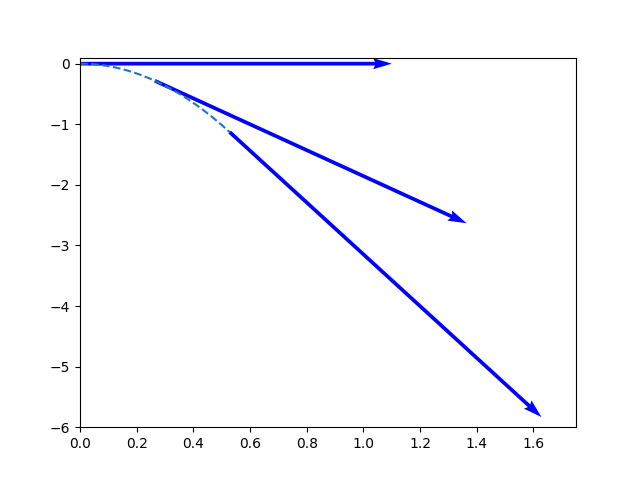
\includegraphics[scale=0.65]{3_09.png} \notag
    \end{align}
\end{problem}

\clearpage

\begin{problem}{3.11}
    Crickets Chirpy and Milada jump from the top of a vertical cliff.
    Chirpy drops downward and reaches the ground in 2.70 s, while Milada jumps horizontally with an initial speed of 95.0 cm/s.
    How far from the base of the cliff will Milada hit the ground?
    Ignore air resistance.

    \solution
    \begin{align}
        v_{0x} &= 95.0 \cms \left(\frac{1 \m}{100 \cm}\right) = 0.950 \mps \\
        x &= x_0 + v_{0x} t = \left(0.950 \mps\right) \left(2.70 \s\right) \approx 2.57 \m
    \end{align}
\end{problem}

\begin{problem}{3.13}
    \textbf{Leaping the River I.} During a storm, a car traveling on a level horizontal road comes upon a bridge that has washed out.
    The driver must get to the other side, so he decides to try leaping the river with his car.
    The side of the road the car is on is 21.3 m above the river, while the opposite side is only 1.8 m above the river.
    The river itself is a raging torrent 48.0 m wide.
    (a) How fast should the car be traveling at the time it leaves the road in order just to clear the river and land safely on the opposite side?
    (b) What is the speed of the car just before it lands on the other side?

    \solution
    \begin{align}
        \Part{a}
        y &= \frac{1}{2} \, gt^2 \\
        \left(21.3 \m - 1.8 \m\right) &= -\frac{1}{2} \left(9.80 \mps^2\right) t^2 \\
        t &= \sqrt{\frac{2 \left(21.3 \m - 1.8 \m\right)}{9.80 \mps^2}} \approx 2.00 \s \\
        x &= x_0 + v_{0x} t \\
        \left(48.0 \m\right) &= v_{0x} \left(1.99 \s\right) \\
        v_{0x} &= \frac{48.0 \m}{1.99 \s} = 24.1 \mps
        \Part{b}
        v_x &= v_{0x} = 24.1 \mps \\
        v_y &= v_{0y} - gt = - \left(9.80 \mps^2\right) \left(2.00 \s\right) = -19.6 \mps \\
        \magnitude{v} &= \sqrt{\left(24.1 \mps\right)^2 + \left(-19.6 \mps\right)^2} \approx 31.0 \mps
    \end{align}
\end{problem}

\clearpage

\begin{problem}{3.15}
    Inside a starship at rest on the earth, a ball rolls off the top of a horizontal table and lands a distance $D$ from the foot of the table.
    This starship now lands on the unexplored Planet X.
    The command, Captain Curious, rolls the same ball off the same table with the same initial speed as on earth and finds that it lands a distance $2.76D$ from the foot of the table.
    What is the acceleration due to gravity on Planet X?

    \solution
    \begin{align}
        \shortintertext{Earth:}
        x &= v_{0x} t \\
        y &= \frac{1}{2} \, gt^2 \\
        t &= \sqrt{\frac{2y}{g}} \\
        x &= v_{0x} \sqrt{\frac{2y}{g}}
        \shortintertext{Planet X:}
        2.76x &= v_{0x} t \\
        t &= \sqrt{\frac{2y}{g}} \\
        2.76x &= v_{0x} \sqrt{\frac{2y}{g}}
        \shortintertext{Divide.}
        \frac{2.76x}{x} &= \frac{v_{0x} \sqrt{\frac{2y}{g_x}}}{v_{0x} \sqrt{\frac{2y}{g_e}}} \\
        2.76 &= \sqrt{\frac{g_e}{g_x}} \\
        2.76 \sqrt{g_x} &= \sqrt{g_e} \\
        \sqrt{g_x} &= \frac{\sqrt{g_e}}{2.76} \\
        g_x &= \left(\frac{\sqrt{g_e}}{2.76}\right)^2 \\
        &\approx 1.28 \mps^2
    \end{align}
\end{problem}

\clearpage

\begin{problem}{3.17}
    A major leaguer hits a baseball so that it leaves the bat at a speed of 30.0 m/s and at an angle of 36.9$^\circ$ above the horizontal.
    Ignore air resistance.
    (a) At what \textit{two} times is the baseball at a height of 10.0 m above the point at which it left the bat?
    (b) Calculate the horizontal and vertical components of the baseball's velocity at each of the two times calculated in part (a).
    (c) What are the magnitude and direction of the baseball's velocity when it returns to the level at which it left the bat?

    \solution
    \begin{align}
        \Part{a}
        x &= \left(v_0 \cos{\alpha_0}\right) t = \left(\left(30.0 \mps\right) \cos{\left(36.9^\circ\right)}\right) t \\
        y &= \left(v_0 \sin{\alpha_0}\right) t - \frac{1}{2} \, gt^2 \\
        &= \left(\left(30.0 \mps\right) \sin{\left(36.9^\circ\right)}\right) t - \frac{1}{2} \left(9.8 \mps^2\right) t^2 \\
        10.0 \m &= \left(\left(30.0 \mps\right) \sin{\left(36.9^\circ\right)}\right) t - \frac{1}{2} \left(9.8 \mps^2\right) t^2 \\
        0 &= \frac{1}{2} \left(9.8 \mps^2\right) t^2 - \left(\left(30.0 \mps\right) \sin{\left(36.9^\circ\right)}\right) t + 10.0 \m \\
        t &= \frac{\left[\left(30.0 \mps\right) \sin{\left(36.9^\circ\right)}\right] \pm \sqrt{\left[- \left(30.0 \mps\right) \sin{\left(36.9^\circ\right)}\right]^2 - 4 \left[\frac{1}{2} \left(9.8 \mps^2\right)\right] \left(10.0 \m\right)}}{2 \left[\frac{1}{2} \left(9.8 \mps^2\right)\right]} \\
        &\approx 0.682 \s \text{ and} \approx 2.99 \s
        \Part{b}
        \vec{v}_x &= v_0 \cos{\alpha_0} = \left(30.0 \mps\right) \cos{\left(36.9^\circ\right)} \approx 24.0 \mps \\
        \vec{v}_{y1} &= v_0 \cos{\alpha_0} - gt = \left(30.0 \mps\right) \sin{\left(36.9^\circ\right)} - \left(9.80 \mps^2\right) \left(0.682 \s\right) \approx 11.3 \mps \\
        \vec{v}_{y2} &= v_0 \cos{\alpha_0} - gt = \left(30.0 \mps\right) \sin{\left(36.9^\circ\right)} - \left(9.80 \mps^2\right) \left(2.99 \s\right) \approx -11.3 \mps
        \Part{c}
        \magnitude{\vec{v}} &= \sqrt{{\vec{v}_x}\phantom{}^2 + {\vec{v}_y}\phantom{}^2} = \sqrt{\left(24.0 \mps\right)^2 + \left(-11.3 \mps\right)^2} \approx 26.5 \mps \\
        \alpha &= \arctan{\left(\frac{\vec{v}_y}{\vec{v}_x}\right)} \approx -25^\circ \text{ or } 25^\circ \text{ under the horizontal.}
    \end{align}
\end{problem}

\clearpage

\begin{problem}{3.19}
    \textbf{Win the Prize.} In a carnival booth, you can win a stuffed giraffe if you toss a quarter into a small dish.
    The dish is on a shelf above the point where the quarter leaves your hand and is a horizontal distance of 2.1 m from this point (\textbf{Fig. E3.19}).
    If you toss the coin with a velocity of 6.4 m/s at an angle of 60$^\circ$ above the horizontal, the coin will land in the dish.
    Ignore air resistance.
    (a) What is the height of the shelf above the point where the quarter leaves your hand?
    (b) What is the vertical component of the velocity of the quarter just before it lands in the dish?

    \solution
    \begin{align}
        \Part{a}
        x &= \left(v_0 \cos{\alpha_0}\right) t \\
        2.1 \m &= \left(\left(6.4 \mps\right) \cos{\left(60^\circ\right)}\right) t \\
        t &= \frac{2.1 \m}{\left(6.4 \mps\right) \cos{\left(60^\circ\right)}} \approx 0.656 \s \\
        y &= \left(v_0 \sin{\alpha_0}\right) t - \frac{1}{2} \, gt^2 \\
        &= \left(\left(6.4 \mps\right) \cos{\left(60^\circ\right)}\right) \left(0.656 \s\right) - \frac{1}{2} \left(9.80 \mps^2\right) \left(0.656 \s\right)^2 \\
        &\approx 1.5 \m
        \Part{b}
        \vec{v}_y &= v_0 \sin{\alpha_0} - gt \\
        &= \left(6.4 \mps\right) \sin{60^\circ} - \left(9.80 \mps^2\right) \left(0.656 \s\right) \approx -0.89 \mps \\
    \end{align}
\end{problem}

\begin{problem}{3.21}
    A man stands on the roof of a 15.0-m-tall building and throws a rock with a speed of 30.0 m/s at an angle of 33.0$^\circ$ above the horizontal.
    Ignore air resistance.
    Calculate
    (a) the maximum height above the roof that the rock reaches;
    (b) the speed of the rock just before it strikes the ground; and
    (c) the horizontal range from the base of the building to the point where the rock strikes the ground.
    (d) Draw $x$-$t$, $y$-$t$, $v_x$-$t$, and $v_y$-$t$ graphs for the motion.

    \solution
    \begin{align}
        \Part{a}
        v_x &= v_0 \cos{\alpha_0} = \left(30.0 \mps\right) \cos{\left(33.0^\circ\right)} \approx 25.2 \mps \\
        v_y &= v_0 \sin{\alpha_0} - gt = \left(30.0 \mps\right) \sin{\left(33.0^\circ\right)} - \left(9.80 \mps^2\right) t \\
        0 &= \left(30.0 \mps\right) \sin{\left(33.0^\circ\right)} - \left(9.80 \mps^2\right) t \\
        t &= \frac{\left(30.0 \mps\right) \sin{\left(33.0^\circ\right)}}{9.80 \mps^2} \approx 1.667 \s \\
        y &= \left(v_0 \sin{\alpha_0}\right) t - \frac{1}{2} \, gt^2 \\
        &= \left(\left(30.0 \mps\right) \sin{\left(33.0^\circ\right)}\right) \left(1.667 \s\right)  - \frac{1}{2} \left(9.80 \mps^2\right) \left(1.667 \s\right)^2 \\
        &\approx 13.6 \m
    \end{align}
    \begin{align}
        \Part{b}
        &\text{Using trial and error, I found } t_f \text{ to be approximately 4.1 s. } \notag \\
        &\text{(After trying so many calculations, I gave up.)} \notag \\
        v_y &= v_0 \sin{\alpha_0} - gt = \left(30.0 \mps\right) \sin{\left(33.0^\circ\right)} - \left(9.80 \mps\right) \left(4.1 \s\right) \approx -23.8 \mps \\
        \magnitude{v} &= \sqrt{{v_x}^2 + {v_y}^2} = \sqrt{\left(25.2 \mps\right)^2 + \left(-23.8 \mps\right)^2} \approx 34.6 \mps
        %-15.0 \m &= \left(\left(30.0 \mps\right) \sin{\left(33.0^\circ\right)}\right) t - \frac{1}{2} \left(9.80 \mps^2\right) t^2 \\
        %0 &= \frac{1}{2} \left(9.80 \mps^2\right) t^2 - \left(\left(30.0 \mps\right) \sin{\left(33.0^\circ\right)}\right) t - 15.0 \m \\
        %t &= \frac{\left(\left(30.0 \mps\right) \sin{\left(33.0^\circ\right)}\right) \pm \sqrt{\left[\left(30.0 \mps\right) \sin{\left(33.0^\circ\right)}\right] - 4 \left[\frac{1}{2} \left(9.80 \mps^2\right)\right]^2 \left(-15.0 \m\right)}}{2 \left[\frac{1}{2} \left(9.80 \mps^2\right)\right]} \\
        %t &\approx -0.894 \s \text{ or } t \approx 34.2 \s
    \end{align}
    \begin{align}
        \Part{c}
        x &= \left(v_0 \cos{\alpha_0}\right) t = \left(30.0 \mps\right) \cos{\left(33.0^\circ\right)} \left(4.1 \s\right) \approx 103 \m
    \end{align}
   \begin{align*}
        \Part{d}
        &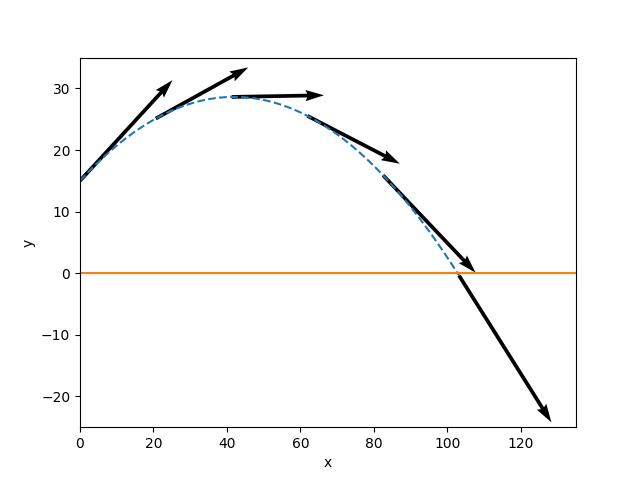
\includegraphics[scale=0.65]{3_21.png}
    \end{align*}
\end{problem}

\end{document}

